\section{Performance Regression Analysis}
\label{src:regression}
Creating multiple symmetric memory partitions results in
multiple symmetric heaps on each PE. The symmetric heap maintenance
includes memory registration with NIC.% and offset maintenance on
%each PE.
Though upcoming communication layers like
libfabrics~\cite{libfabrics} have support for Scalable memory
Registration, Cray SHMEM implementation over DMAPP uses basic memory
registration. Hence there is an increase in memory footprint on
DMAPP on maintaining symmetric heaps on each PE.

\vspace{-20pt}
\begin{algorithm}[!h]
\begin{algorithmic}
    \Procedure{\texttt{shmem\_putmem}}
    {void *dest, const void *src, size\_t nblks, int pe\_id}\;
        dmapp\_seg\_desc\_t *target\_seg = \texttt{NULL}\;
        dmapp\_type\_t type = \texttt{DMAPP\_BYTE}\;
        \If {\normalfont (dest.segment $\equiv$
                         \texttt{DATA\_SEGMENT})} {
            target\_seg = \texttt{DATA\_SEGMENT}\;
            \tcp{verify if dest buffer is a static or global variable}
        } \ElseIf {\normalfont (dest.segment $\equiv$
                         \texttt{SHEAP\_SEGMENT})} {
            target\_seg = \texttt{SHEAP\_SEGMENT}\;
            \tcp{verify if dest buffer is in default symmetric heap}
        } \Else {
            segment\_identified = \textit{false}\;
            \For {\normalfont (int i = 1; i $\leq$ N; i++)}{
                \If{\normalfont (dest.segment $\equiv$
                    \texttt{USER\_SEGMENT\_i})} {
                    target\_seg = \texttt{USER\_SEGMENT\_i})\;
                    segment\_identified = \textit{true}\;
                }
            }
            \If{\normalfont(segment\_identified $\equiv$
                    \textit{false})} {
                abort()\;
            }
            \tcp{search through all partitions to match the symmetric heap}
        }
        dmapp\_put(dest, target\_seg, pe\_id, src, nelems, type)\;
        return\;
    \EndProcedure
    \caption{Lookup logic with N symmetric memory partitions per PE}
    \label{algo:normal-lookup}
\end{algorithmic}
\end{algorithm}
\vspace{-20pt}

%Apart from increase in memory footprint on memory registration,
Identifing the correct symmetric segment is essential before
performing an
underlying communication operation. %with symmetric heap lookup on each
%RMA and AMO operation is expected to introduce performance
%regression.
Algorithm~\ref{algo:normal-lookup} shows the introduction of lookup
logic trying to match the correct symmetric heap segment on the
\texttt{shmem\_putmem} operation. Similar, lookups are introduced in
all OpenSHMEM RMA and AMO operations. \texttt{USER\_SEGMENT} refers to
the symmetric heap segments created on user-defined memory partitions.

\begin{figure*}[h!]
    \vspace{-30pt}
    \centering
    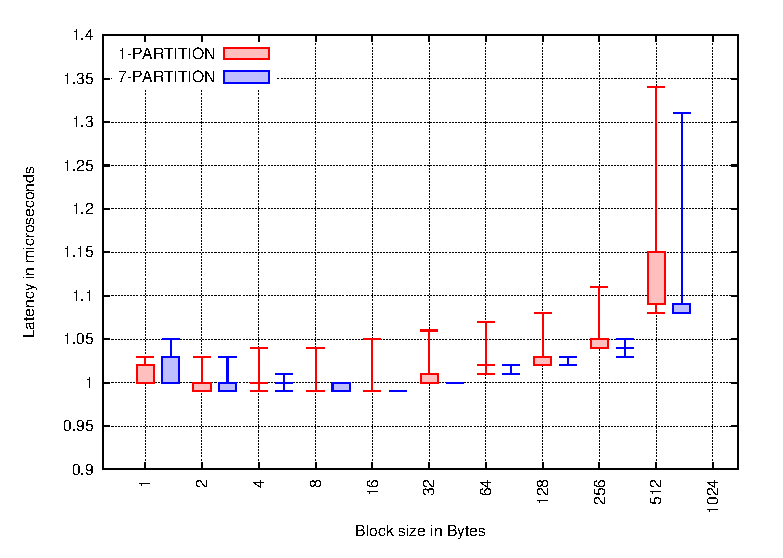
\includegraphics[width=\linewidth]{graph/osu-put.eps}
    \caption{Performance difference on using destination buffers
    from 1 partition against 7 partitions on the modified OSU Put
    microbenchmark}
    \label{graph:lookup}
    \vspace{-20pt}
\end{figure*}

We measured the performance regression behind this additional lookup
operation using a modified OSU microbenchmark~\cite{osu-mb}
on a Cray XC system with Intel KNL processors. To measure the average
latency on every \texttt{shmem\_putmem} operation, we used 2 nodes
with 1 PE per node.
The normal OSU microbenchmark selects the buffer from the either
\texttt{DATA\_SEGMENT} or \texttt{SHEAP\_SEGMENT}
per job. We modified the benchmark by creating
one destination buffer for \texttt{N} partitions and randomly select
the destination buffer from different partitions for every iteration.
We timed the average performance of all iterations.% of the
%\texttt{shmem\_putmem} operation.

Figure~\ref{graph:lookup} shows the
performance difference between using 1 and 7 partitions on very small
data sizes. The average performance variations is around 2\% to
3\%. This can be attributed as noise. If we increase
the number of partitions to 127, we could see variations as high
as 6\%. But, we expect users to create only one partition per
memory kind.
%and not \texttt{N} unnecessary partitions.
Moreover, as mentioned in
Table~\ref{tab:const} the \texttt{SHMEMX\_MAX\_PARTITIONS} library
constant in Cray SHMEM is 7.

We observe similar performance variation on small data sizes on other
RMA and AMO operations. For larger message sizes, the segment lookup
does not contribute for any performance variation.

\section{Performance Analysis}
\label{src:perf}

\begin{figure*}[h!]
%    \vspace{-30pt}
    \centering
    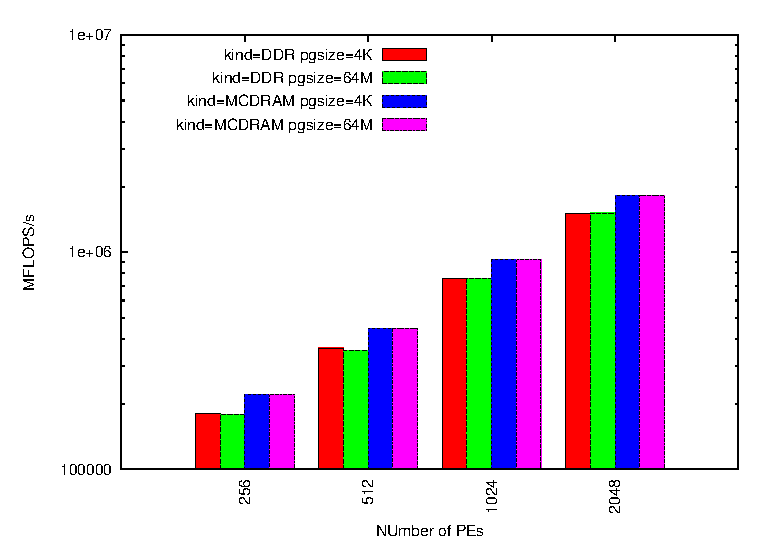
\includegraphics[width=\linewidth]{graph/2d-stencil.eps}
    \caption{Performance difference on using different kinds of memory
    and different hugepages on ParRes 2D-Stencil SHMEM kernels}
    \label{graph:2dstencil}
%    \vspace{-20pt}
\end{figure*}

